In addition to finding jets in the tracking system, we can take advantage of ECCE's calorimetry systems for jet analysis.  Like in the tracking analysis, this was done with 18x275 GeV Pythia 8 electron proton collisions with a $Q^2>100\hbox{ GeV}^2$ on the prop.4 configuration.  Once again, the anti-$k_T$ jet finding algorithm was used with a jet radius $R=0.5$ with the constraint $z<0.95$.  

To improve the collection of energy in the calorimeters, the towers are group together with clustering algorithms to try to make each cluster contain all the energy of a particle.  Two algorithms in particular have been utilized in this analysis, V3 and MA clustering.  \todo{expand}


\begin{figure}
    \centering
    \begin{subfigure}{0.4\textwidth}
        \centering
        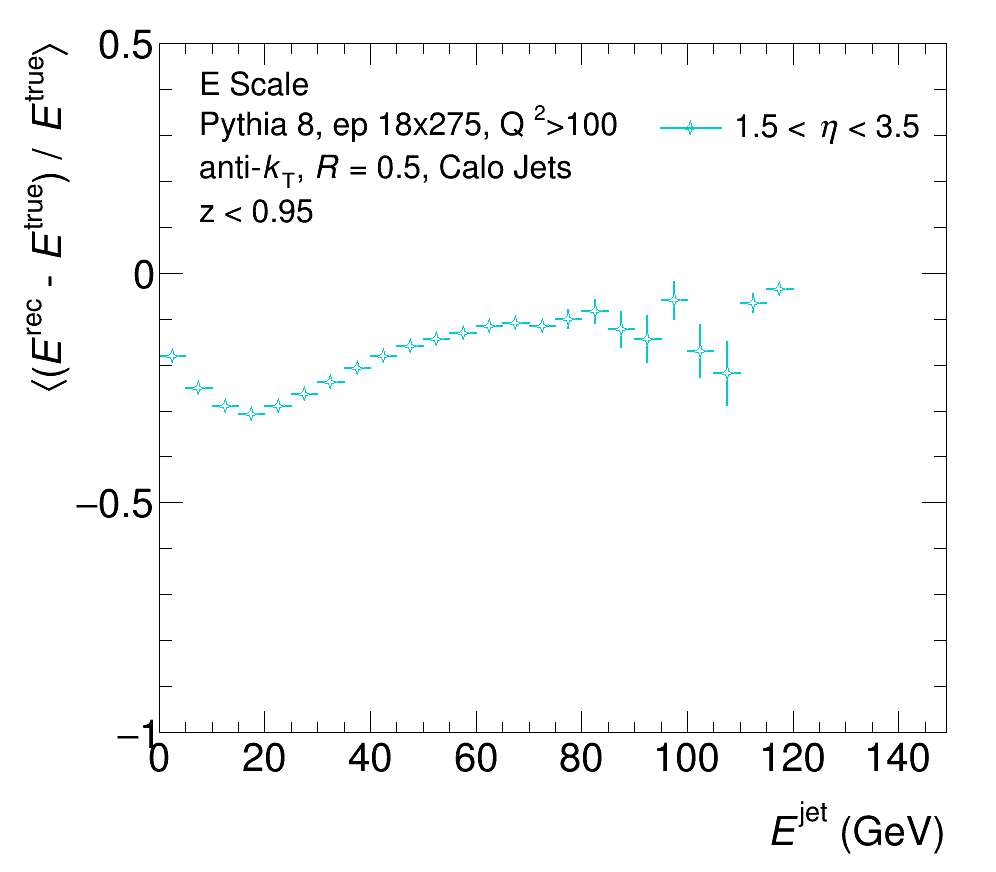
\includegraphics[width=\linewidth]{figs/jet_plots/JES_calo_grouped.png}
        \caption{Calorimetry jets scale}
        \label{fig:calo_energy_scale}
    \end{subfigure}
    \hfill
    \begin{subfigure}{0.4\textwidth}
        \centering
        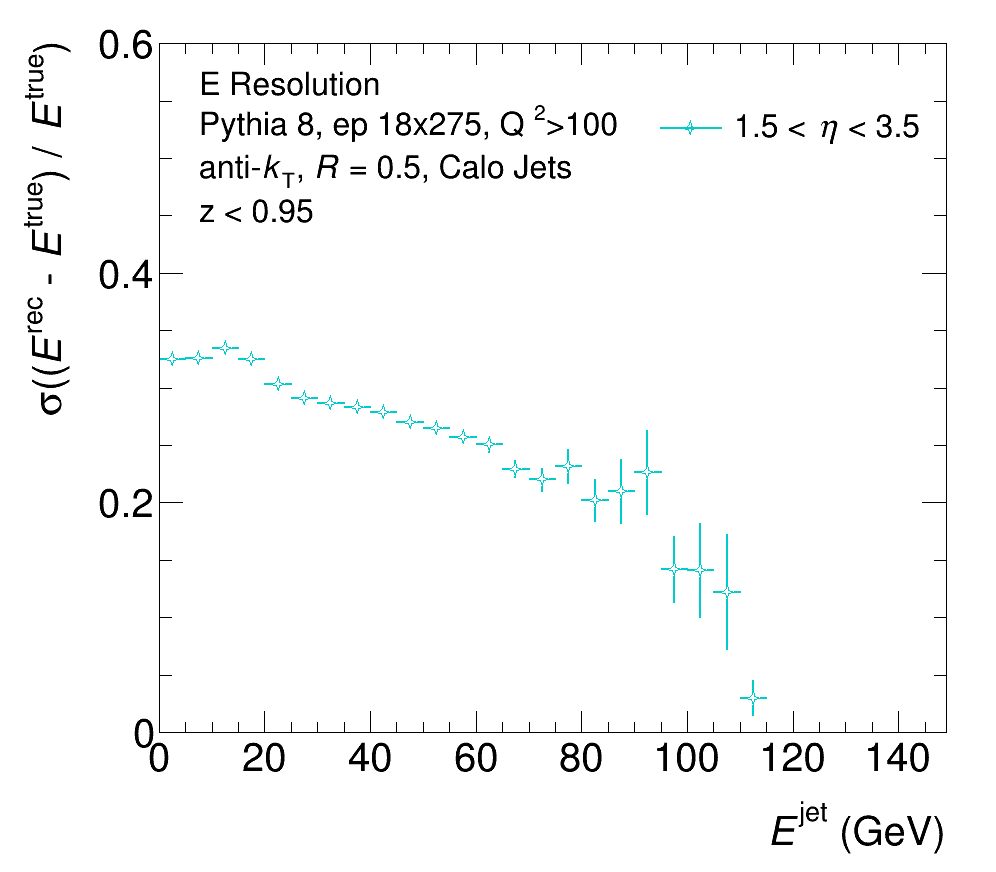
\includegraphics[width=\linewidth]{figs/jet_plots/JER_E_calo_grouped.png}
        \caption{Calorimetry jet resolution}
        \label{fig:calo_energy_resolution}
    \end{subfigure}
    \caption{The scale and resolution of the energy of calorimetry jets.}
    \label{fig:calo_energy_reso_scale}
\end{figure}



\begin{figure}
    \centering
    \begin{subfigure}{0.4\textwidth}
        \centering
        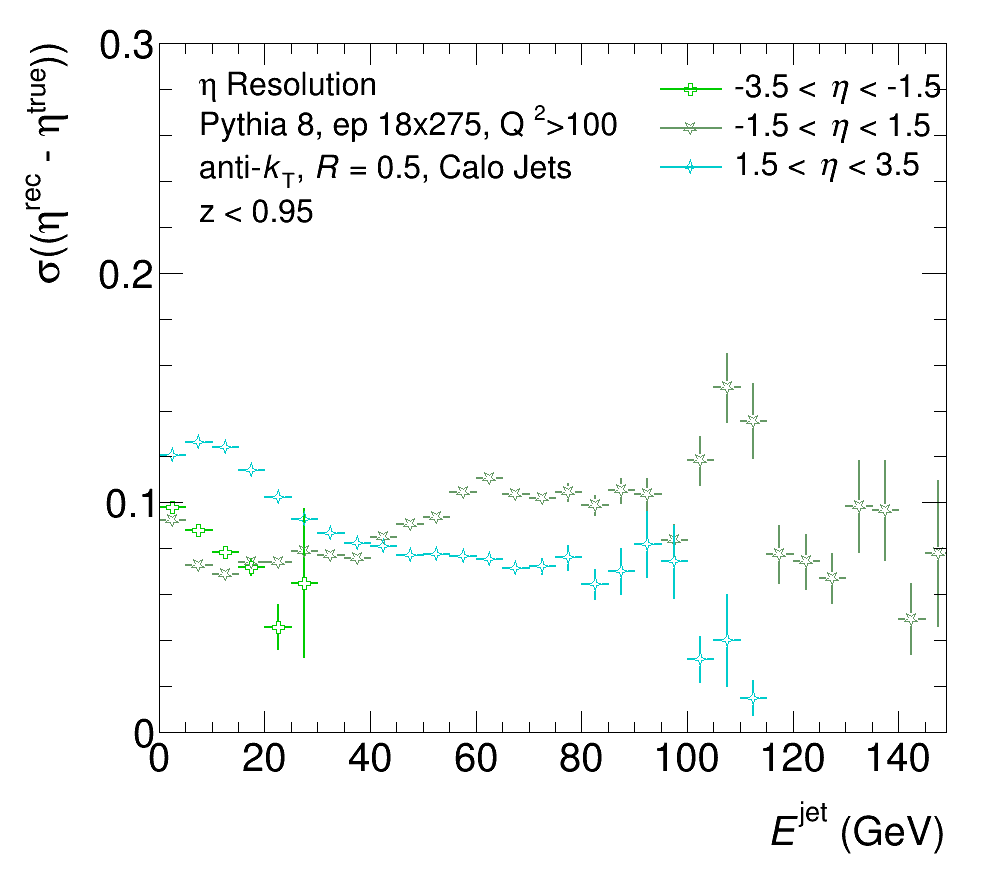
\includegraphics[width=\linewidth]{figs/jet_plots/EtaReso_calo_grouped.png}
        \caption{Calorimetry jet $\eta$ resolution}
        \label{fig:calo_eta_resolution}
    \end{subfigure}
    \hfill
    \begin{subfigure}{0.4\textwidth}
        \centering
        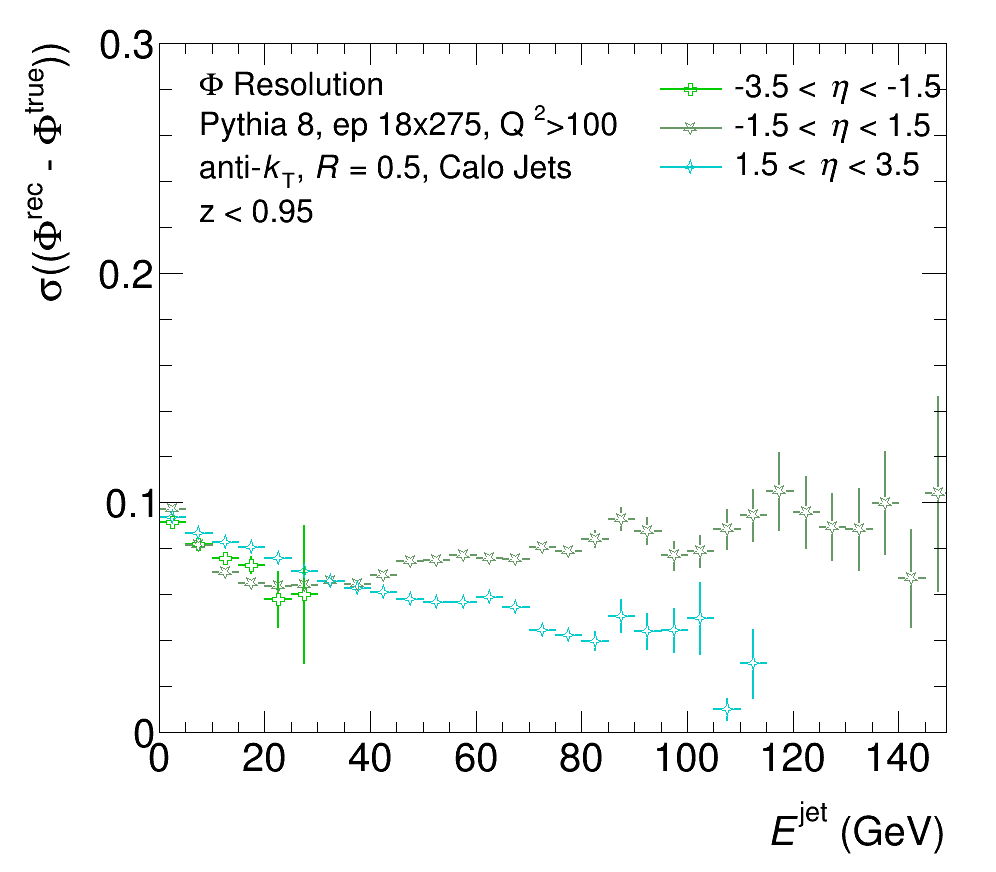
\includegraphics[width=\linewidth]{figs/jet_plots/PhiReso_calo_grouped.png}
        \caption{Calorimetry jet $\phi$ resolution}
        \label{fig:calo_phi_resolution}
    \end{subfigure}
    \caption{The spatial resolution of calorimetry jets}
    \label{fig:calo_spatial_reso_scale}
\end{figure}